\documentclass{article}

%
% 引入模板的style文件
%
\usepackage{homework}

\setCJKmainfont{SimSun}[AutoFakeBold] %宋体加粗
\setCJKsansfont{SimHei}[AutoFakeBold] %黑体加粗


\usepackage{minted} %配合minted宏包进行好看的高亮
\usepackage{currfile} %配合minted宏包进行好看的高亮
\usepackage{caption} %配合minted宏包进行好看的高亮
\usepackage{tcolorbox} %配合minted宏包进行好看的高亮
\usepackage{xcolor} %配合minted宏包进行好看的高亮
\tcbuselibrary{skins} %配合minted宏包进行好看的高亮
\tcbuselibrary{minted} %配合minted宏包进行好看的高亮
\usemintedstyle{paraiso-dark} %配合minted宏包进行好看的高亮
\usepackage{framed} 
\usepackage{amsmath}


%
% 封面
%


\title{
	
\includegraphics[width=0.6\textwidth]{images/title/ucas_logo 1.pdf}\\
    \vspace{1in}
    \textmd{\textbf{\hmwkClass}}\\
	\textmd{\Large{\textbf{\hmwkClassID}}}\\
    \textmd{\textbf{\hmwkTitle}}\\
    \normalsize\vspace{0.1in}\large{\hmwkCompleteTime }\\
    \vspace{0.1in}\large{\textit{\hmwkClassInstructor\ }}\\
    \vspace{1in}
	
\includegraphics[width=0.25\textwidth]{images/title/Cyber.jpg}\\
	\vspace{1in}
}

\author{
	\hmwkAuthorName \\ 
	\hmwkAuthorStuID \\
	\hmwkAuthorInst \\
	\hmwkAuthorzhuanye \\
	\hmwkAuthorfangxiang
	}
\date{}

\renewcommand{\part}[1]{\textbf{\large Part \Alph{partCounter}}\stepcounter{partCounter}\\}


%
% 正文部分
%
\begin{document}


\maketitle


%\include{chapters/ch01}
%\include{chapters/ch02}
%\include{chapters/ch03}
%\include{chapters/ch04}
%\include{chapters/ch05}


\pagebreak



\begin{homeworkProblem}
	假设对称旅行商问题的邻接矩阵如下所示, 试用优先队列式分枝限界算法给出最短环游. 画出状态空间树的搜索图, 并说明搜索过程.
	$$
	\left( \begin{matrix}
		\infty&		20&		30&		10&		11\\
		&		\infty&		16&		4&		2\\
		&		&		\infty&		6&		7\\
		&		&		&		\infty&		12\\
		&		&		&		&		\infty\\
	\end{matrix} \right)
	$$
	\begin{figure}[H]
		\centering
		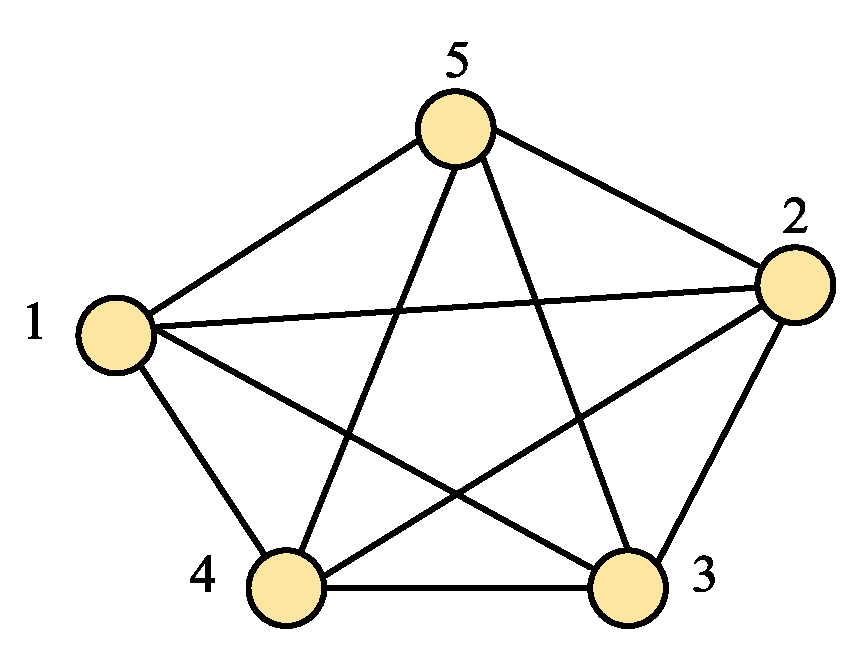
\includegraphics[width=0.3\textwidth]{images/title/旅行商问题.pdf}
		\caption{旅行商问题}
		\label{fig:旅行商问题}
	\end{figure}
	\solution 状态空间树的搜索图如下图\ref{fig:解空间树搜索图}中所示:
	\begin{figure}[H]
		\centering
		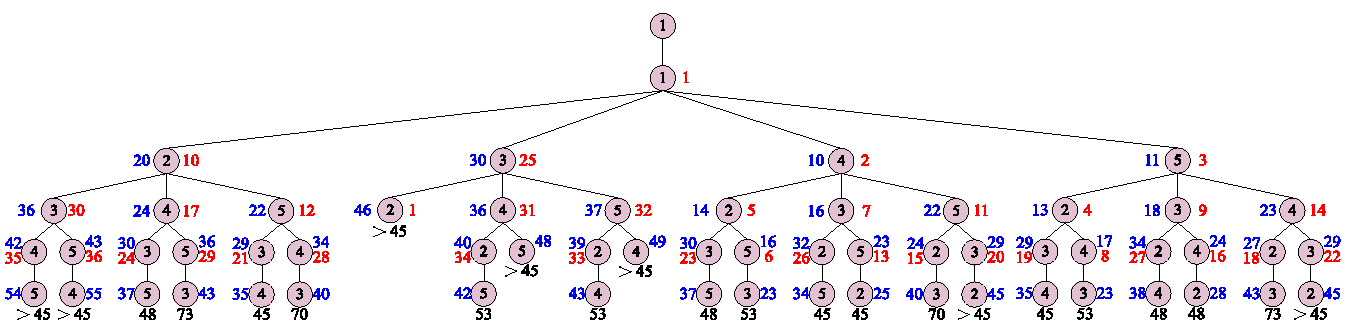
\includegraphics[width=1.0\textwidth]{images/title/解空间树搜索图.pdf}
		\caption{解空间树搜索图}
		\label{fig:解空间树搜索图}
	\end{figure}
	图中圆圈内为顶点序号, 蓝色数字为该路径到该节点的总路程, 红色数字表示该节点的搜索序数. 从顶点1开始搜索, 将其4个儿子节点放入队列. 然后优先访问队列中当前路程最小的节点, 再将它的儿子放入队列. 然后重复上述过程, 优先访问队列中当前路径最小的节点, 将其儿子放入队列. 第一个被访问到的叶子节点为1-4-2-5-3-1这条路径, 总路程为53, 记录当前最短路径. 之后若某节点的路径大于最短路程, 则不再搜索该节点的子树. 若某叶子节点的总路程小于当前最短路径, 则更新之. 如此搜索, 当访问到1-4-3-5-2-1这条路径的叶子节点时, 其总路程为$45<53$, 将45更新为当前最短路径, 继续搜索. 最后得出最短环游为1-2-5-3-4-1、1-4-3-2-5-1、1-4-3-5-2-1、1-5-2-3-4-1, 总路程均为45.
\end{homeworkProblem}


\pagebreak





\begin{homeworkProblem}
	最佳调度问题: 假设有$n $个任务要由$k $个可并行工作的机器来完成, 完成任务$i $需要的时间为$t_i$. 试设计一个分枝限界算法, 找出完成这$n $个任务的最佳调度, 使得完成全部任务的时间(从机器开始加工任务到最后停机的时间)最短.

	\solution 设计的算法步骤如下:
	\begin{itemize}
		\item 先将任务由大到小排序;
		\item 计算$n$个任务需要的总时间和平均到$k$个机器上的时间;
		\item 将大于平均时间的任务各分配一个机器, 找到最大完成时间;
		\item 将其他任务顺序安排在一台机器上, 如果时间超出最大时间, 则把该任务交给下一个机器, 下一个任务继续在这台机器上试安排, 直到所有任务都不能在小于最大完成时间的情况下安排;
		\item 安排下一台机器直到所有任务安排完;
		\item 或有可能安排某些任务找不到小于最大完成时间, 那么重新扫描各台机器使再加上该任务后时间最小, 按此方法安排完所有任务.
	\end{itemize}
\end{homeworkProblem}

\begin{homeworkProblem}
	分派问题: 给$n$个人分派$n$件工作, 给第$i$人分派第$j$件工作的成本是$C(i,j)$, 试用分枝限界法求成本最小的工作分配方案.

	\solution 设$n$个人的集合是$\left\{ 1,2,\cdots,n \right\}$, $n$项工作的集合是$\left\{ 1,2,\cdots,n \right\}$, 每个人恰好1项工作. 于是有
	$$\text{把工作}j\text{分配给}i\Leftrightarrow x_i=j,\quad i,j=1,2,\cdots n
	$$

	设解向量为$X=\left< x_1,x_2,\cdots ,x_n \right>	$, 分配成本为$\displaystyle C\left( X \right) =\sum_{i=1}^n{C\left( i,x_i \right)}	$. 搜索空间是排列树. 部分向量$\left< x_1,x_2,\cdots ,x_k \right> $表示已经考虑了人$1,2,\cdots,k$的工作分配. 节点分支的约束条件为:$$x_{k+1}\in \left\{ 1,2,\cdots ,n \right\} \backslash \left\{ x_1,x_2,\cdots ,x_k \right\} 
	$$

	可以设立代价函数:$$F\left( x_1,x_2,\cdots ,x_k \right) =\sum_{i=1}^k{C\left( i,x_i \right)}+\sum_{i=k+1}^n{\text{min} \left\{ C\left( i,t \right) :t\in \left\{ 1,2,\cdots ,n \right\} \backslash \left\{ x_1,x_2,\cdots ,x_k \right\} \right\}}
	$$
	界$B$是已得到的最好可行解的分配成本. 如果代价函数大于界, 则回溯. 算法的时间复杂度为$O(n\cdot n!)$.
\end{homeworkProblem}

\pagebreak


\begin{homeworkProblem}
	如图\ref{fig:Latin方}所示, 一个4阶Latin方是一个$4\times 4$的方格, 在它的每个方格内填入$1,2,3$或4, 并使得每个数字在每行、每列都恰好出现一次. 用回溯法求出所有第一行为1,2,3,4的所有4阶Latin方. 将每个解的第2行到第4行的数字从左到右写成一个序列. 如图\ref{fig:Latin方}中的解是$\left<3,4,1,2,4,3,2,1,2,1,4,3\right>$. 给出所有可能的4阶Latin方.
	\begin{figure}[H]
		\centering
		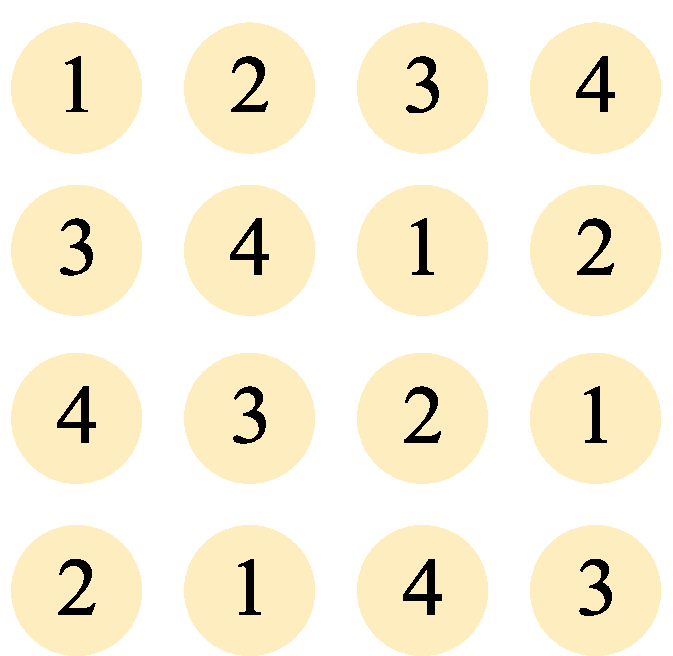
\includegraphics[width=0.2\textwidth]{images/title/Latin方.pdf}
		\caption{Latin方}
		\label{fig:Latin方}
	\end{figure}
	通过PPT中的回溯算法可以求出共有24个Latin方, 具体如下图\ref{fig:Latin方结果}所示:
	\begin{figure}[H]
		\centering
		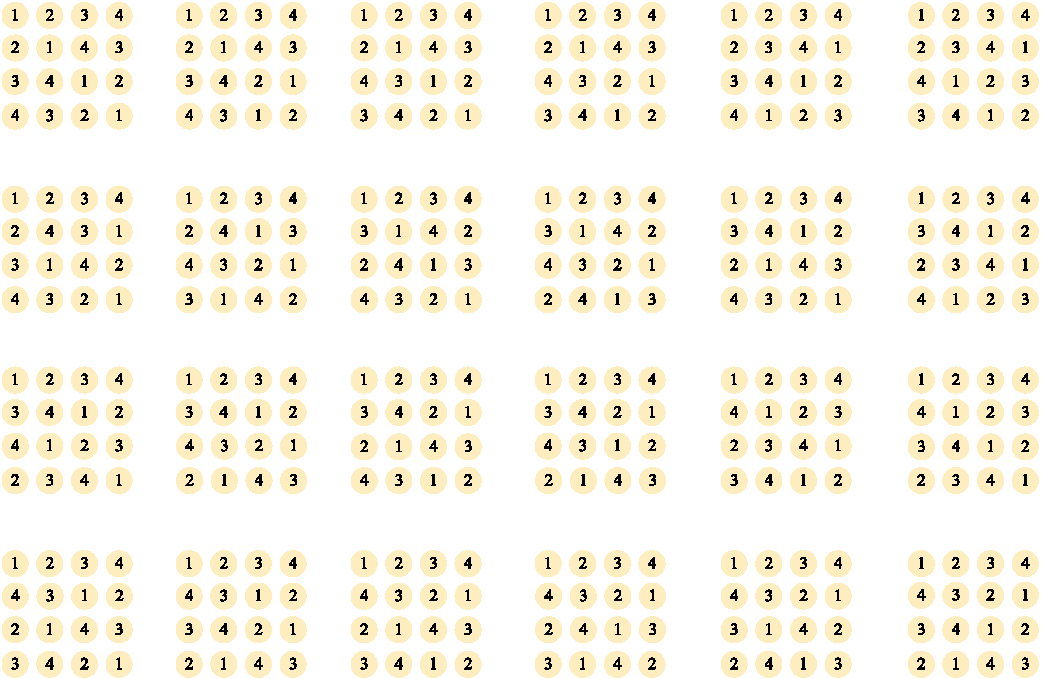
\includegraphics[width=1.0\textwidth]{images/title/Latin方结果.pdf}
		\caption{Latin方结果}
		\label{fig:Latin方结果}
	\end{figure}
\end{homeworkProblem}



% 引用文献
\bibliographystyle{unsrt}  % unsrt:根据引用顺序编号
\bibliography{refs}


\end{document}
